Verwenden Sie die Funktion \verb+gsl_sf_hyperg_0F1+ oder ein Programm,
welches die Reihenentwicklung der hypergeometrischen Funktion
$\mathstrut_0F_1$ direkt berechnet, um die
in Aufgabe \ref{501} gefundenen Lösungen der Airy-Differentialgleichung
zu plotten.
\index{Airy-Differentialgleichung}%

\begin{figure}
\centering
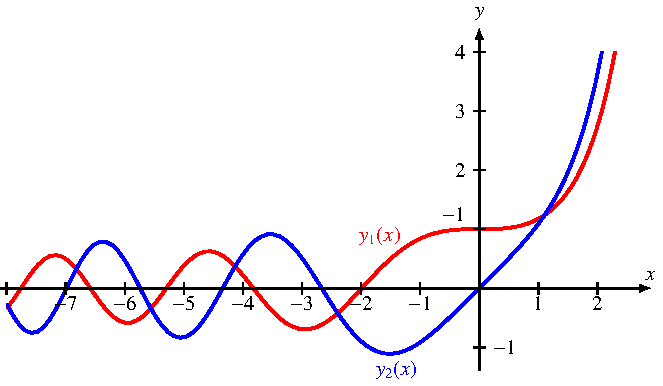
\includegraphics{chapters/050-differential/uebungsaufgaben/airy.pdf}
\caption{Plot der Lösungen der Airy-Differentialgleichung $y''-xy=0$
zu den Anfangsbedingungen $y(0)=1$ und $y'(0)=0$ in {\color{red}rot}
und $y(0)=0$ und $y'(0)=1$ in {\color{blue}blau}.
\label{buch:differentialgleichunge:uebung:503:plot}}
\end{figure}
\begin{loesung}
Die Implementation der hypergeometrische Funktion $\mathstrut_0F_1$ in der
GNU Scientific Library führt $\mathstrut_0F_1$ auf Bessel-Funktionen
\index{GNU Scientific Library}%
\index{Bessel-Funktion}%
zurück, was für $c=\frac23$ nicht möglich ist. 
In diesem Fall ist also eine eigene Implementation nötig.
Die Plots sind in Abbildung~\ref{buch:differentialgleichunge:uebung:503:plot}
dargestellt.
Mehr zur numerischen Berechnung von $\mathstrut_0F_1$ im
Kapitel~\ref{chapter:0f1}.
\end{loesung}
